Imported source material for a section is the raw, pre-\LaTeX{} input that may arrive as markdown, outline notes, or other authoring fragments. It is useful as evidence of intent, but it is not yet the section payload that the compiler consumes. The section payload is the generated \LaTeX{} body for one specific section, written as a durable artifact in its own file and shaped to fit the surrounding manuscript.

This separation matters because the system treats source, transformation, and output as distinct state surfaces. Imported markdown can remain readable and editable as upstream material, while the section payload records the agent's current best rendering of that material in \LaTeX{}. Keeping those layers apart makes it possible to revise prose without overwriting the original source, to compare drafts against their inputs, and to inspect how a section changed over time.

Section agents therefore write only to section-specific \texttt{.tex} files such as \texttt{tex/section\_payloads/ch07\_sec01\_section\_payloads.tex}. That constraint keeps each agent's responsibility local: one agent owns one section payload, and no agent silently mutates the whole document. The result is easier review, clearer attribution, and fewer accidental cross-section edits. It also supports incremental compilation, because a changed section can be regenerated, diffed, and repaired without forcing unrelated sections to be rewritten.

In this workflow, the imported source remains the starting point, but the section payload is the artifact that downstream assembly uses. The payload is what enters proposal records, diffs, build logs, and compiled output. By writing only the section payload, the agent preserves a clean boundary between what was provided, what was inferred, and what is now ready for review.

This design is especially important in a multi-agent manuscript, where several agents may be drafting, revising, checking references, or responding to build feedback at the same time. A section-specific TeX file gives each agent a narrow, inspectable target and prevents the manuscript from becoming an opaque shared buffer. In short, imported markdown is source material; the section payload is the controlled \LaTeX{} realization of that source material; and the section file is the unit of ownership that keeps the system coherent.

That distinction also clarifies the artifact lifecycle described in this chapter. Source notes are not discarded when a section is rendered; they remain available as upstream evidence. The generated payload is the controlled output that can be reviewed, compared, and compiled. Later sections in this chapter extend that same logic to proposals, diffs, and repair loops: once a section exists as a separate payload, it can be tracked as a changeable artifact rather than as an invisible mutation of the manuscript.

Figure~\ref{fig:ch07_sec01_section_payloads} summarizes the distinction between imported source material and the section payload that section agents maintain.

\begin{figure}[htbp]
\centering
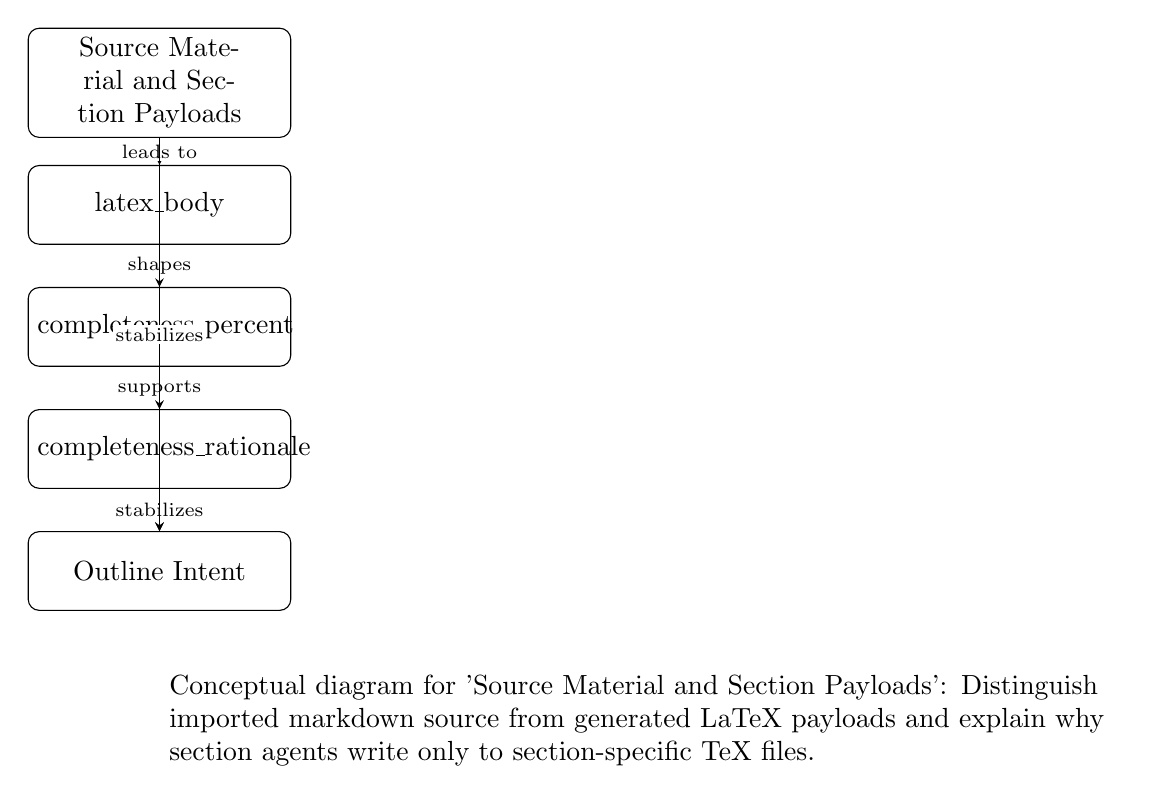
\begin{tikzpicture}[>=stealth, node distance=2.2cm,
  concept/.style={draw, rounded corners, align=center, text width=3.1cm, minimum height=1cm},
  relation/.style={font=\scriptsize, fill=white, inner sep=1pt}]
\node[concept] (n1) at (0,0.0) {Source Material and Section Payloads};
\node[concept] (n2) at (0,-1.55) {latex\_body};
\node[concept] (n3) at (0,-3.1) {completeness\_percent};
\node[concept] (n4) at (0,-4.65) {completeness\_rationale};
\node[concept] (n5) at (0,-6.2) {Outline Intent};
\draw[->] (n1) -- node[relation] {leads to} (n2);
\draw[->] (n2) -- node[relation] {shapes} (n3);
\draw[->] (n3) -- node[relation] {supports} (n4);
\draw[->] (n4) -- node[relation] {stabilizes} (n5);
\draw[->] (n1) -- node[relation] {stabilizes} (n5);
\node[align=left, text width=12cm, anchor=north west] at (0,-7.4) {Conceptual diagram for 'Source Material and Section Payloads': Distinguish imported markdown source from generated LaTeX payloads and explain why section agents write only to section-specific TeX files.};
\end{tikzpicture}

\caption{Conceptual diagram for ``Source Material and Section Payloads'': imported markdown source is distinct from the generated \LaTeX{} payload, and section agents write only to section-specific TeX files.}
\label{fig:ch07_sec01_section_payloads}
\end{figure}
